\documentclass[10pt,a4paper,twocolumn]{IEEEtran}
\usepackage[utf8]{inputenc}
\usepackage{amsmath, amssymb}
\usepackage{newtxtext,newtxmath}
\usepackage{graphicx}
\usepackage{hyperref}
\usepackage{enumitem}
\usepackage{xcolor}
\usepackage{cite}
\usepackage{listings}
\usepackage{tikz}
\usetikzlibrary{shapes, arrows, positioning}
\setlength{\columnsep}{25pt}
\usepackage{float}
\usepackage{caption}
\title{Deterministic, Fair, and Secure Multi-Process WASM Runtime}
\author{Mateus Vital Nabholz \\ Distributed Computing Laboratory, EPFL \\ mateus.vitalnabholz@epfl.ch \\ Spring 2025}
\date{}

\begin{document}

\maketitle

\begin{abstract}
This report presents the design, implementation, and evaluation of a WebAssembly (WASM) runtime capable of running multiple programs concurrently in a fair, deterministic, and secure manner. The runtime features a robust process structure, a scheduler, and a secure file system with sandboxing and disk usage limits. We demonstrate the effectiveness of our approach through a series of targeted experiments and test programs.
\end{abstract}

\section{Introduction}\label{sec:intro}

Replicated execution—where multiple independent machines run the same program state-for-state—provides crash tolerance and verifiable output; this replicated state-machine approach underpins the reliability of modern blockchains and distributed databases~\cite{schneider_smr}.

While many types of programs could benefit from these guarantees—higher availability, transparent audits, and simpler failover—replicated execution is today almost exclusively reserved for smart contracts on blockchains~\cite{ethereum}. These smart contracts, however, operate under severe restrictions: they have only highly restricted, indirect I/O (e.g., via oracles), lack a file system, and do not follow the standard lifetime of conventional programs (e.g., no \texttt{main()} entry point). As a result, it is currently impossible to execute arbitrary programs—with rich I/O, file system access, and standard lifecycles—in a replicated, deterministic, and fair manner.

This work addresses this gap. We design and implement a runtime for the replicated execution of arbitrary programs, with the explicit goal of supporting deployment on public blockchains. This setting requires the ability to execute many programs concurrently, while ensuring strong isolation, determinism, and resource fairness.

To achieve this, we rely on WebAssembly (WASM) as a unified instruction set architecture (ISA) and for its strong compute determinism. However, WASM alone does not provide deterministic I/O, file system semantics, or program lifetime management. Nor does it ensure fair resource allocation among many concurrent programs. Our runtime addresses these challenges by providing:

\begin{enumerate}
    \item \textbf{Deterministic, Fair Multi-Process Scheduling:} The runtime can execute several WASM programs concurrently with deterministic outputs and fair CPU slices, even across blocking system calls.
    \item \textbf{Deterministic I/O and File-System Semantics:} The runtime enforces deterministic I/O and file-system semantics.
    \item \textbf{Standard Process-Lifecycle Management under Replication:} The runtime supports conventional program lifecycles (e.g., \texttt{main()}), enabling arbitrary programs to run under replicated state machine execution.
    \item \textbf{Robust Security and Isolation:} Each process operates within a dedicated sandbox, with strict enforcement of disk usage quotas and file system isolation. Attempts to exceed resource limits or access other sandboxes are reliably prevented.
    \item \textbf{Extensive Testing via Custom WASM Programs:} A suite of test programs was developed to validate determinism, fairness, security, and functionality. These programs exercise the runtime's features and are described in detail in the Implementation section, with results presented in the Evaluation.
\end{enumerate}

In short, we bring replicated, deterministic, and fair execution to arbitrary programs—not just smart contracts—making public blockchains and other distributed systems far more versatile.

\section{Background}\label{sec:background}

This section introduces key concepts and technologies that underpin this project. We explain them here so that later references in the report can be concise.

\subsection{WebAssembly (WASM)}
WebAssembly (WASM) is a low-level, binary instruction format designed for safe, portable, and efficient execution across diverse platforms~\cite{wasm_w3c,wasm_sok,wasm_formal}. Originally developed to enable high-performance applications in web browsers, WASM has since become a popular compilation target for a variety of programming languages, including C, C++, and Rust. Its sandboxed execution model, deterministic semantics, and support for system interface standards (such as WASI) make it an attractive foundation for secure, cross-platform application deployment---including blockchain and serverless environments. In this project, WASM serves as the execution format for user programs, enabling strong isolation and portability.

\subsection{Blockchain Consensus}
Consensus protocols are fundamental to blockchains, ensuring that distributed participants agree on the order and content of transactions~\cite{bitcoin,blockchain_tutorial}. Early blockchains like Bitcoin used proof-of-work, but modern systems often employ Byzantine Fault Tolerant (BFT) consensus (e.g., PBFT, Tendermint) to achieve finality and resilience against malicious actors~\cite{castro_liskov_pbft,tendermint}. Consensus is critical for replicated execution: it ensures that all honest nodes process the same sequence of transactions, which is essential for determinism and security. Our runtime is designed for future integration with a BFT-based blockchain (Chop Chop), and thus must support deterministic, verifiable execution.

\subsection{Replicated State Machines}
The replicated state machine (RSM) paradigm is a classic approach to building fault-tolerant distributed systems~\cite{schneider_smr,bonomi_smr}. In RSM, a set of nodes each maintain a copy of the system state and apply the same sequence of deterministic operations, as agreed by consensus. This ensures consistency even in the presence of failures or adversarial behavior. Blockchains can be viewed as large-scale RSMs, where each block encodes a batch of operations. Deterministic execution is crucial: any divergence in state due to nondeterminism can lead to consensus failure. Our WASM runtime is explicitly designed to support RSM-style replicated execution, with strong determinism guarantees.

\subsection{Droplet Compiler}
The Droplet compiler, developed for the Chop Chop blockchain, is an ahead-of-time (AOT) compiler that compiles WebAssembly (WASM) code to native code via LLVM IR. Unlike proof-producing compilers, Droplet focuses on providing automatic cooperative multi-threading support through a \texttt{yield()} function, and implements µsection-based multi-threading, enabling the deterministic execution of batches of threads with shared memory. At the time of writing, the Droplet compiler has not yet been publicly released.

\subsection{Coarse-Grained Cooperative Multithreading}
The runtime implements coarse-grained, cooperative multithreading with a round-robin scheduler~\cite{tannenbaum_os}: a process runs until it hits a long-latency system call or an explicit yield(), at which point the scheduler switches to the next ready process. Context switches only occur at these well-defined "pit stops"—not on a timer or hardware interrupt—so the grain is coarse. Yielding is cooperative: a process must voluntarily yield, otherwise it can monopolize the CPU. In the future, the compiler will automate yield insertion to ensure fairness without programmer intervention.

\subsection{Other Relevant Concepts}
\textbf{Deterministic Execution:} Determinism is the property that a program, given the same inputs and environment, always produces the same outputs. In replicated and blockchain systems, determinism is essential to ensure that all nodes reach the same state. Nondeterminism can lead to forks or consensus failures~\cite{batch_schedule_execute}.

\textbf{Permissioned Blockchains:} Unlike public blockchains, permissioned blockchains restrict participation to a known set of entities. This allows for more efficient consensus protocols (e.g., BFT) and is common in enterprise and research settings~\cite{blockchain_tutorial,bonomi_smr}.

\section{Design}\label{sec:design}

\textbf{Key Terms:}
\begin{itemize}
    \item \textbf{Runtime:} The overall program that manages the pool of WASM processes, scheduling, isolation, etc.; runs as a single OS process.
    \item \textbf{WASM Process:} A user program (e.g., C or Rust compiled to .wasm) managed by the runtime; runs in its own thread with its own WASM engine instance and resources.
    \item \textbf{WASM Engine:} The engine/interpreter (e.g., Wasmtime, Wasmer) that executes a single WASM program; each WASM process has its own WASM engine instance.
\end{itemize}

The runtime itself is a single OS process that manages all WASM processes, providing the scheduler, consensus communication, and system call mediation. Each WASM process runs as a thread within this runtime instance.

The design of our WASM runtime centers on providing a robust, fair, and secure environment for executing multiple untrusted programs concurrently. The architecture is guided by the following key principles:

\subsection*{WASM Processes, Threads, and Isolation}
In this context, a \textbf{WASM process} refers to a single WASM program executed in its own OS thread, with a dedicated WASM engine instance and isolated resources (such as a file system sandbox and resource limits). All WASM processes are managed by the same runtime, but are strictly isolated from each other by the WASM engine, which enforces separate memory spaces and file system sandboxes. Threads themselves do not provide isolation; rather, they are a technical means to allow our runtime to manage multiple WASM engine instances—one per WASM process—within a single OS process. This approach is necessary because each individual WASM engine instance (e.g., an interpreter or engine) is designed to execute a single program at a time.

\begin{itemize}
    \item At any moment, only one WASM process is allowed to execute.
    \item When a WASM process reaches a long-latency system call (e.g., file I/O, network, or explicit yield), the system call blocks and waits for the scheduler to allow it to continue.
    \item The scheduler selects which process may continue; all others remain loop-locked at their last system call.
    \item This ensures deterministic execution: even though all threads are alive at the OS level, only one makes progress in the runtime at a time.
\end{itemize}

\textbf{Execution Flow:}
\begin{verbatim}
For each WASM process:
  Upon reaching long-latency system call:
    Pause execution
    Notify scheduler
    Wait until selected to continue
  When selected by scheduler:
    Resume execution
\end{verbatim}

\subsection*{Runtime as Process Manager}
The runtime acts as a central manager for all WASM processes, scheduling, monitoring, and controlling them to ensure system-wide properties such as determinism, fairness, and security. Each WASM program is launched as a separate WASM process, with its own dedicated thread and isolated resources.

\subsection*{Per-Process Isolation}
To prevent interference and ensure strong security, each WASM process is fully isolated from the others. This is achieved through:
\begin{itemize}
    \item \textbf{WASM Engine Isolation:} Each WASM process runs in its own WASM engine instance, which enforces strict separation of memory and resources; threads themselves do not provide isolation.
    \item \textbf{Thread-per-Process Model:} Each WASM process runs in its own OS thread, managed at a high level by the runtime, but ultimately scheduled and managed by the operating system. The runtime ensures that each thread waits in a loop whenever its state is not \texttt{Running}, resuming execution only when the scheduler sets its state back to \texttt{Running}.
    \item \textbf{Sandboxed File System:} Every WASM process is assigned a unique sandbox directory. All file operations are restricted to this directory, preventing access to other WASM processes' data or the host system.
    \item \textbf{Crash Containment:} If a WASM process crashes or behaves maliciously, the runtime detects the failure and cleans up the process without affecting others. This ensures that faults are contained and do not propagate.
\end{itemize}

\begin{figure}[h]
    \centering
    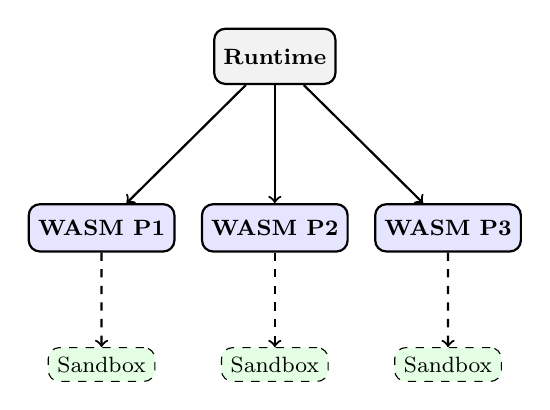
\begin{tikzpicture}[scale=0.7, every node/.style={font=\footnotesize}]
        % Runtime
        \node[draw, thick, rounded corners, minimum width=1.5cm, minimum height=0.7cm, fill=gray!10] (runtime) {\textbf{Runtime}};
        % WASM Processes
        \foreach \i in {1,2,3} {
            \node[draw, thick, rounded corners, minimum width=0.8cm, minimum height=0.6cm, fill=blue!10, below=1.5cm of runtime, xshift={(\i-2)*2.2cm}] (proc\i) {\textbf{WASM P\i}};
            \draw[->, thick] (runtime) -- (proc\i);
        }
        % Sandboxes
        \foreach \i in {1,2,3} {
            \node[draw, dashed, rounded corners, minimum width=0.9cm, minimum height=0.3cm, fill=green!10, below=1.2cm of proc\i] (sb\i) {Sandbox};
            \draw[->, thick, dashed] (proc\i) -- (sb\i);
        }
    \end{tikzpicture}
    \caption{Each WASM process is fully isolated: it runs in its own thread and WASM engine instance, has a dedicated file descriptor table, and operates within a private sandbox directory.}
    \label{fig:process-isolation}
\end{figure}

\subsection*{Threat Model}
We assume that each WASM process may be buggy or malicious, attempting to escape its sandbox, exceed resource limits, or interfere with other processes. The runtime, operating system, and underlying hardware are trusted. Our security mechanisms are designed to prevent WASM processes from accessing files or resources outside their assigned sandbox, exceeding their disk quota, or affecting the execution or data of other WASM processes. We do not defend against vulnerabilities in the runtime itself, attacks on the host operating system or hardware, or side-channel attacks. Denial-of-service attacks that exhaust system-wide resources (e.g., CPU, memory) are out of scope.

\subsection*{Security Goals and Defenses}
\begin{center}
\small
\begin{tabular}{|p{1.5cm}|p{1.9cm}|p{1.3cm}|p{1.25cm}|}
\hline
\textbf{Asset / Threat} & \textbf{Attack Surface} & \textbf{High-Level Defense} & \textbf{Residual Risk} \\
\hline
File system isolation & File system syscalls & Per-process sandbox & Low \\
\hline
Disk quota enforcement & File/directory writes & Disk-usage accounting & Low \\
\hline
Process isolation & Memory, syscalls & Separate WASM engines & Depends on WASM engine correctness \\
\hline
Fair CPU allocation & Scheduler & Round-robin at yield points & Depends on yield placement \\
\hline
Crash containment & Process panics & Per-process error handling & Low \\
\hline
\end{tabular}
\captionof{table}{Security goals, attack surfaces, high-level defenses, and residual risks in the runtime.}
\end{center}
\vspace{0.5em}

\subsection*{System Calls as Control and Security Checkpoints}
All interactions between WASM programs and the host are mediated by a set of custom system calls. These system calls serve two main purposes:
\begin{itemize}
    \item \textbf{Execution Control:} System calls act as "pit-stops" where the runtime can check whether a process should continue running, block, or yield. This enables the scheduler to maintain control over process execution and enforce fairness.
    \item \textbf{Security Enforcement:} Before delegating to the underlying host system call, the runtime checks that the operation respects all security policies. This includes verifying that file operations remain within the sandbox and that disk usage does not exceed per-process quotas.
\end{itemize}

\begin{figure}[h]
    \centering
    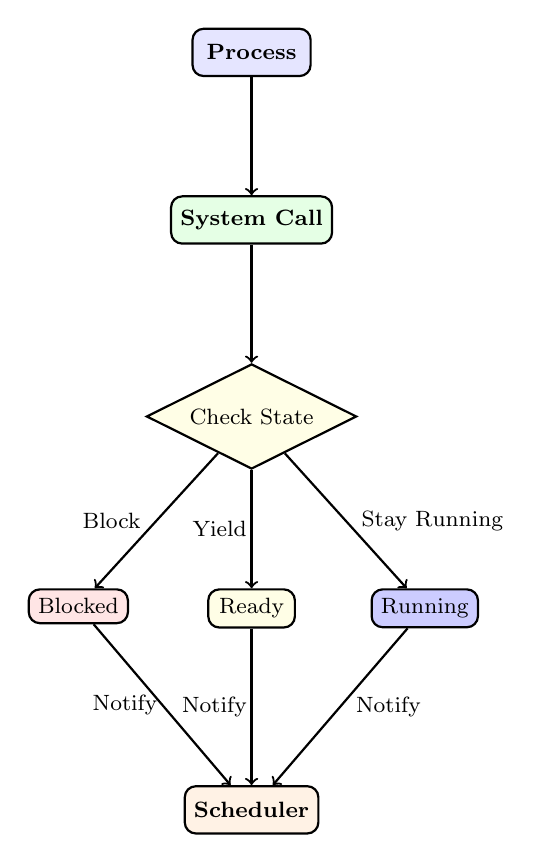
\begin{tikzpicture}[node distance=1.5cm, every node/.style={font=\footnotesize}]
        % Process
        \node[draw, thick, rounded corners, minimum width=1.5cm, minimum height=0.6cm, fill=blue!10] (proc) {\textbf{Process}};
        % System Call
        \node[draw, thick, rounded corners, minimum width=1.5cm, minimum height=0.6cm, fill=green!10, below=of proc] (syscall) {\textbf{System Call}};
        % Decision
        \node[draw, diamond, thick, aspect=2, fill=yellow!10, below=of syscall] (check) {Check State};
        % Blocked
        \node[draw, thick, rounded corners, minimum width=1.1cm, minimum height=0.4cm, fill=red!10, below=of check, xshift=-2.2cm] (blocked) {Blocked};
        % Ready
        \node[draw, thick, rounded corners, minimum width=1.1cm, minimum height=0.4cm, fill=yellow!10, below=of check] (ready) {Ready};
        % Running
        \node[draw, thick, rounded corners, minimum width=1.1cm, minimum height=0.4cm, fill=blue!20, below=of check, xshift=2.2cm] (running) {Running};
        % Scheduler
        \node[draw, thick, rounded corners, minimum width=1.5cm, minimum height=0.6cm, fill=orange!10, below=4cm of check] (sched) {\textbf{Scheduler}};
        % Arrows
        \draw[->, thick] (proc) -- (syscall);
        \draw[->, thick] (syscall) -- (check);
        \draw[->, thick] (check) -- node[left, xshift=-2pt] {Block} (blocked);
        \draw[->, thick] (check) -- node[right, xshift=2pt] {Stay Running} (running);
        \draw[->, thick] (check) -- node[left, xshift=2pt] {Yield} (ready);
        \draw[->, thick] (blocked) -- node[left, xshift=2pt] {Notify} (sched);
        \draw[->, thick] (ready) -- node[left, xshift=2pt] {Notify} (sched);
        \draw[->, thick] (running) -- node[right, xshift=2pt] {Notify} (sched);
    \end{tikzpicture}
    \caption{System calls can set the process to Blocked, Ready, or leave it Running, and notify the scheduler as appropriate.}
    \label{fig:syscall-state}
\end{figure}

\subsection*{Fairness and Determinism via Scheduling}
To ensure that all processes make progress and that execution is repeatable, the runtime provides a mechanism for round-robin scheduling at explicit yield points. Currently, yield points must be inserted manually in each program, so fairness depends on the frequency and placement of these yields. In the future, the Droplet compiler will automate yield insertion, enabling coarse-grained and transparent round-robin scheduling. Thus, the runtime enforces fairness at yield points, but the overall fairness policy will depend on the compiler's yield insertion strategy.

\subsection*{Philosophy and Validation}
The overarching philosophy is to provide a runtime that is both secure and predictable, making it suitable for deployment in decentralized and adversarial environments. By combining strong isolation, resource accounting, and deterministic scheduling, the design supports reliable execution of untrusted code. The effectiveness of these design choices is validated through a comprehensive suite of test programs, ranging from simple to complex, as described in the Evaluation section.

\section{Implementation}\label{sec:implementation}

\subsection*{Structs and Data Structures}
\begin{lstlisting}[language=Rust, caption={Key Structs: Process, ProcessData, ProcessState}, label={lst:structs}, basicstyle=\ttfamily\scriptsize, frame=single]
// runtime/src/runtime/process.rs
#[derive(Debug, Clone, Copy, PartialEq)]
pub enum ProcessState {
    Ready,
    Running,
    Blocked,
    Finished,
}

#[derive(Debug, Clone)]
pub enum BlockReason {
    StdinRead,
    Timeout {
        resume_after: u64
    },
    FileIO,
    WriteIO(String),
    NetworkIO,
}

#[derive(Clone)]
pub struct ProcessData {
    pub state: Arc<Mutex<ProcessState>>,
    pub cond: Arc<Condvar>,
    pub block_reason: Arc<Mutex<
        Option<BlockReason>
    >>,
    pub fd_table: Arc<Mutex<FDTable>>,
    pub root_path: PathBuf,
    pub max_disk_usage: u64,
    pub current_disk_usage: Arc<Mutex<u64>>,
    pub write_buffer: Arc<Mutex<Vec<u8>>>,
    pub max_write_buffer: usize,
    pub id: u64,
    pub next_port: Arc<Mutex<u16>>,
    pub network_queue: Arc<Mutex<Vec<
        OutgoingNetworkMessage
    >>>,
    pub nat_table: Arc<Mutex<
        NatTable
    >>,
    pub args: Vec<String>,
}

pub struct Process {
    pub id: u64, // Unique process ID
    pub thread: thread::JoinHandle<()>,
    pub data: ProcessData,
}
\end{lstlisting}

\subsection*{Process Structure}
The core of the runtime is the \texttt{Process} struct, which encapsulates all state and resources for a running program. Each process maintains:
\begin{itemize}
    \item \textbf{Identifiers and Paths:} A unique process ID and a root path for sandboxed file operations.
    \item \textbf{State Management:} A \texttt{state} field (protected by a mutex) that tracks whether the process is \texttt{Running}, \texttt{Ready}, \texttt{Blocked}, or \texttt{Finished}. A condition variable (\texttt{cond}) is used to signal state changes between the scheduler and the process.
    \item \textbf{Thread Handle:} Each process runs in its own thread, referenced by the \texttt{thread} field.
    \item \textbf{File Descriptor Table:} The \texttt{fd\_table} manages open files and directories, mapping WASI file descriptors to host resources.
    \item \textbf{Disk Usage Tracking:} Fields for current and maximum disk usage, used to enforce per-process quotas.
    \item \textbf{Write Buffer:} A buffer for pending writes, supporting non-blocking IO and efficient flushing.
    \item \textbf{Block Reason:} An optional field indicating why a process is blocked (e.g., waiting for IO, timeout, or file system operation).
    \item \textbf{Networking Fields:} (e.g., network queue, NAT table) are present in \texttt{ProcessData} for networked programs. [See Perello Mas~\cite{perellomas2025} for networking and consensus details.]
\end{itemize}
Additionally, in \texttt{start\_process}, we handle the case where a process panics, ensuring that a failure in one process does not cause the entire runtime to panic. This separation ensures that faults are contained and do not propagate to other WASM processes, improving overall robustness.

\subsection*{System Calls and Process Control}
System calls are implemented to mediate all interactions between WASM programs and the host. Key system calls for process control include:
\begin{itemize}
    \item \texttt{fd\_read} and \texttt{fd\_write}: Handle reading from and writing to files and standard streams. \texttt{fd\_write} uses a per-process buffer to ensure fairness: writes are buffered and only flushed when the buffer is full or explicitly requested, so no single process can monopolize IO. \texttt{fd\_read} blocks the process if the requested size is too large or if no input is available, ensuring that processes do not starve others.
    \item \texttt{path\_open}, \texttt{path\_create\_directory}, \texttt{path\_unlink\_file}, \texttt{path\_remove\_directory}: All file and directory operations are checked to ensure they remain within the process's sandbox. This is enforced by the methods \texttt{usage\_add}, \texttt{usage\_sub}, and path checks in \texttt{fs.rs} (e.g., \texttt{wasi\_path\_open}, \texttt{wasi\_path\_create\_directory}, \texttt{wasi\_path\_unlink\_file}, \texttt{wasi\_path\_remove\_directory}). Disk usage is tracked and enforced on every operation.
    \item \texttt{proc\_exit}: Marks the process as \texttt{Finished} and notifies the scheduler for cleanup.
    \item \texttt{wasi\_\_builtin\_rt\_yield}: Implements cooperative yielding. When called, it sets the process state to \texttt{Ready}, notifies the scheduler, and waits until the scheduler schedules it again. This is implemented in \texttt{builtin\_yield.rs} and is essential for enabling round-robin scheduling and fairness among processes.
\end{itemize}
Blocking is handled by updating the process's state and block reason, then waiting on the condition variable until the scheduler unblocks the process.

\subsection*{Scheduling and Blocking}
\begin{figure}[h]
    \centering
    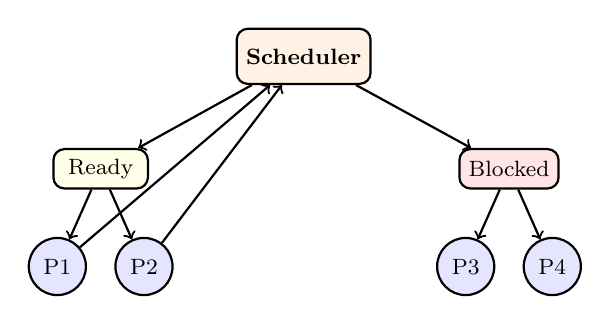
\begin{tikzpicture}[scale=0.7, every node/.style={font=\footnotesize}]
        % Scheduler
        \node[draw, thick, rounded corners, minimum width=1.7cm, minimum height=0.7cm, fill=orange!10] (sched) {\textbf{Scheduler}};
        % Queues
        \node[draw, thick, rounded corners, minimum width=1.2cm, minimum height=0.5cm, fill=yellow!10, below left=0.8cm and 1.1cm of sched] (ready) {Ready};
        \node[draw, thick, rounded corners, minimum width=1.2cm, minimum height=0.5cm, fill=red!10, below right=0.8cm and 1.1cm of sched] (blocked) {Blocked};
        % Processes
        \foreach \i in {1,2} {
            \node[draw, thick, circle, fill=blue!10, below=0.6cm of ready, xshift={(\i-1.5)*1.1cm}] (p\i) {P\i};
            \draw[->, thick] (ready) -- (p\i);
            \draw[->, thick] (p\i) -- (sched);
        }
        \foreach \i in {3,4} {
            \node[draw, thick, circle, fill=blue!10, below=0.6cm of blocked, xshift={(\i-3.5)*1.1cm}] (p\i) {P\i};
            \draw[->, thick] (blocked) -- (p\i);
        }
        % Arrows
        \draw[->, thick] (sched) -- (ready);
        \draw[->, thick] (sched) -- (blocked);
    \end{tikzpicture}
    \caption{The scheduler manages ready and blocked queues, dispatching processes and handling state transitions.}
    \label{fig:scheduler-operation}
\end{figure}

The scheduler (\texttt{scheduler.rs}) manages all process execution. It maintains two queues: a ready queue for processes that can run, and a blocked queue for those waiting on IO or other events. The main scheduling loop:
\begin{itemize}
    \item Sets a process to \texttt{Running} and signals it to proceed.
    \item Waits for the process to yield, block, or finish (using the condition variable and state field).
    \item Moves the process to the appropriate queue based on its new state.
    \item If there are no ready processes, the scheduler first checks blocked processes to see if their block reason has been resolved (e.g., IO is now available, timeout expired, or file system operation completed). If no processes become ready after this, it processes the next batch from consensus input to update process states or add new processes. [See Perello Mas~\cite{perellomas2025} for networking and consensus details.]
    \item When a process finishes, its thread is joined and its sandbox directory is deleted.
\end{itemize}
This design ensures fair and deterministic scheduling, as well as strict isolation and cleanup for each process. The use of \texttt{wasi\_\_builtin\_rt\_yield} allows processes to voluntarily yield control, enabling a round-robin scheduling policy.


\subsection*{IO System Calls}
The IO system calls in \texttt{fs.rs} and \texttt{fd.rs} provide the interface between WASM programs and the host file system. Key features include:
\begin{itemize}
    \item \textbf{Sandbox Enforcement:} All file paths are resolved relative to the process's root path, and path checks prevent escape from the sandbox. This is implemented in methods such as \texttt{wasi\_path\_open}, \texttt{wasi\_path\_create\_directory}, \texttt{wasi\_path\_unlink\_file}, and \texttt{wasi\_path\_remove\_directory}.
    \item \textbf{Disk Usage Accounting:} Every file and directory operation updates the process's disk usage using \texttt{usage\_add} and \texttt{usage\_sub}. Operations that would exceed the quota are denied with an appropriate error code.
    \item \textbf{Buffered Writes:} Writes are buffered and only flushed to disk when the buffer is full or explicitly requested, supporting efficient non-blocking IO and fairness among processes.
    \item \textbf{Blocking Semantics:} If a read or write cannot proceed (e.g., waiting for input, buffer full), the process is blocked and the scheduler is notified. When the condition is resolved, the scheduler unblocks the process and it resumes execution.
    \item \textbf{File Descriptor Management:} The \texttt{fd\_table} tracks all open files and directories, supporting standard WASI operations like \texttt{fd\_read}, \texttt{fd\_write}, \texttt{fd\_seek}, and \texttt{fd\_close}.
\end{itemize}

\subsection*{Test Program Implementations}
To validate the runtime, we implemented a suite of test programs in \texttt{wasm\_programs/}. These include:
\begin{itemize}
    \item Programs for testing disk limits (\texttt{test\_disk\_limit}, \texttt{test\_many\_small\_files}, \texttt{test\_many\_empty\_files}), sandbox isolation (\texttt{test\_cross\_sandbox\_access}, \texttt{test\_escape\_sandbox}, \texttt{test\_symlink}), and file system operations (\texttt{mkdir\_test}, \texttt{test\_rmdir}, \texttt{test\_unlink}, \texttt{read\_dir}).
    \item Programs that exercise process scheduling and fairness (\texttt{simple\_yield}, \texttt{simple\_block}, \texttt{simple\_write}, \texttt{simple\_yield\_block}), including explicit yielding and blocking.
    \item Server programs (\texttt{image\_server}, \texttt{kv\_server}) to test persistent storage and system call correctness.
\end{itemize}
The results of these experiments are discussed in detail in the Evaluation section.

\section{Evaluation}\label{sec:evaluation}

The following evaluation addresses all the main contributions described in the Introduction, including deterministic and fair scheduling, deterministic I/O and file-system semantics, process-lifecycle management, robust security and isolation, and comprehensive testing.

\subsection{Experimental Setup}
All experiments were conducted on a MacBook Air M3 with 24~GB of RAM, running macOS 14.4. The WASM runtime and all test programs were compiled using \texttt{wasm32-wasi-clang} with the provided Makefile in the \texttt{wasm\_programs} directory.

\subsection{Test Programs}
The following test programs were used to validate the runtime:
\begin{itemize}
    \item \textbf{simple\_yield, simple\_block, simple\_write, simple\_yield\_block:} Simple programs to test concurrent execution, blocking, and yielding.
    \item \textbf{test\_disk\_limit, test\_many\_small\_files, test\_many\_empty\_files:} Programs that attempt to exceed disk usage limits in various ways.
    \item \textbf{test\_cross\_sandbox\_access, test\_escape\_sandbox, test\_symlink:} Programs that attempt to breach sandbox isolation or perform disallowed operations.
    \item \textbf{image\_server, kv\_server, network\_server, network\_test, netcat, posix:} Server and network programs to test file system and network functionality in realistic scenarios.
    \item \textbf{mkdir\_test, test\_rmdir, test\_unlink, test\_write\_block, read\_dir, hello:} Programs to test standard file system operations.
\end{itemize}

\subsection{Determinism and Fairness}
To evaluate determinism and fairness, we conducted a series of experiments:
\begin{itemize}
    \item \textbf{Simple concurrent execution:} We ran two simple programs (e.g., \texttt{simple\_yield} and \texttt{simple\_block}) concurrently. The output was consistent across repeated runs, confirming determinism.
    \item \textbf{Multiple simple programs with minimal blocking:} Several simple programs (e.g., \texttt{simple\_yield}, \texttt{simple\_block}, \texttt{simple\_write}, \texttt{simple\_yield\_block}) were run together. Their execution order and results remained consistent, demonstrating fairness and determinism.
    \item \textbf{Complex programs with network and IO blocking:} We ran the simple programs alongside more complex ones (e.g., \texttt{image\_server}, \texttt{kv\_server}, \texttt{network\_server}, \texttt{network\_test}) that perform network and IO operations, as well as programs that yield (e.g., \texttt{simple\_yield\_block}). The scheduler maintained fairness and determinism even under these conditions.
\end{itemize}
In these experiments, yield points were manually inserted at reasonable locations in the test programs to demonstrate fairness under the round-robin scheduler.

\subsection{Security: Disk Usage Limits and Sandboxing}
We validated the enforcement of security policies through the following experiments:
\begin{itemize}
    \item \textbf{Disk usage limit:} We ran programs that attempted to exceed their disk quota in different ways:
    \begin{itemize}
        \item A program that writes a large file at once (\texttt{test\_disk\_limit}).
        \item A program that writes many small files (\texttt{test\_many\_small\_files}).
        \item A program that creates many empty files (\texttt{test\_many\_empty\_files}).
    \end{itemize}
    In all cases, the runtime correctly stopped further writes after the disk limit was reached.
    \item \textbf{Sandbox isolation:} We ran multiple programs simultaneously and verified that each had its own isolated sandbox for all file operations. Programs attempting to access another program's sandbox (\texttt{test\_cross\_sandbox\_access}, \texttt{test\_escape\_sandbox}) failed to do so, confirming effective isolation.
    \item \textbf{Malicious program test:} We included a malicious program that tried to access another program's sandbox. The runtime blocked these attempts, and no unauthorized access occurred.
\end{itemize}

\subsection*{Security Validation: Mapping Defenses to Tests}
The following list maps each security defense to the experiment(s) that validate it:
\begin{itemize}
    \item \textbf{File system isolation:} Validated by \texttt{test\_cross\_sandbox\_access}, \texttt{test\_escape\_sandbox}, and \texttt{test\_symlink} (all blocked as expected).
    \item \textbf{Disk quota enforcement:} Validated by \texttt{test\_disk\_limit}, \texttt{test\_many\_small\_files}, \texttt{test\_many\_empty\_files} (writes stop at quota).
    \item \textbf{Process isolation:} Validated by running multiple programs in parallel; no interference observed.
    \item \textbf{Fair CPU allocation:} Validated by concurrent execution of \texttt{simple\_yield}, \texttt{simple\_block}, \texttt{simple\_write}, \texttt{simple\_yield\_block} (outputs are fair and deterministic; yield points were manually inserted in these tests).
    \item \textbf{Crash containment:} Validated by intentionally crashing a process; others continue unaffected.
\end{itemize}

\subsection{Functionality: File System and Program Isolation}
We tested the correctness and isolation of the file system as follows:
\begin{itemize}
    \item \textbf{Standard read/write operations:} Each program was able to perform standard file operations (create, read, write, delete) within its own sandbox, as validated by \texttt{mkdir\_test}, \texttt{test\_rmdir}, \texttt{test\_unlink}, \texttt{test\_write\_block}, and \texttt{read\_dir}.
    \item \textbf{Server programs:} We ran the \texttt{image\_server} and \texttt{kv\_server} to ensure that data was properly stored in their respective sandboxes and that system calls worked as expected.
    \item \textbf{Sandbox deletion:} We ran a short-lived program (\texttt{simple\_yield}) alongside longer-running ones (\texttt{kv\_server}, \texttt{image\_server}) and confirmed that its sandbox was deleted upon termination, while the others remained unaffected.
\end{itemize}

\subsection{Summary of Results}
\begin{itemize}
    \item \textbf{Determinism:} All runs produced identical output, confirming deterministic scheduling.
    \item \textbf{Security:} All breaching attempts failed; disk limits and sandboxing were strictly enforced.
    \item \textbf{Functionality:} All standard file operations worked as intended; each program had isolated, persistent storage within its quota.
\end{itemize}

\section{Related Work}\label{sec:related}

This project was developed as a duo, with the overall runtime architecture, process isolation, and system call logic described in this report, and the networking and consensus/runtime interaction implemented and evaluated by Ricardo Perello Mas. For a detailed discussion of the networking stack, consensus input, and distributed execution, see the companion report by Perello Mas~\cite{perellomas2025}.

\section{Conclusion}\label{sec:conclusion}

This work presents a WASM runtime that advances the state of the art in deterministic, fair, and secure multi-process execution. By combining strong per-process isolation, robust resource accounting, and a round-robin scheduler with explicit yield support, the runtime achieves reliable and repeatable execution of untrusted programs. The comprehensive suite of test programs demonstrates that the system enforces strict security policies, maintains fairness, and provides correct file system semantics for each process.

The design and implementation choices made in this project lay a solid foundation for future work. In particular, the runtime is well-positioned for integration with decentralized platforms such as the Chop Chop blockchain, where determinism, isolation, and security are paramount. 

Future directions include:
\begin{itemize}
    \item \textbf{Automating yield insertion:} Integrating compiler support (e.g., via Droplet) to automatically insert yield points, ensuring fairness and preemptability without requiring manual intervention by the programmer.
    \item \textbf{Extending system call support:} Broadening the set of supported WASI system calls to enable a wider range of applications and improve compatibility with existing software.
    \item \textbf{Improving performance:} Reducing runtime overhead, optimizing the scheduler, and minimizing context-switching costs to achieve higher throughput and lower latency.
    \item \textbf{Adding multi-threading support:} Enabling concurrency within WASM processes, making runtime compatible with multi-threaded programs.
    \item \textbf{User-level threads for WASM processes:} Ideally, each WASM process would be implemented as a user-level thread (green thread or coroutine) rather than an OS thread. This would allow the runtime to efficiently manage process states and avoid wasting OS resources when a process is blocked in a loop, as OS threads continue to be scheduled by the operating system even when not making progress. User-level threads would enable more scalable and resource-efficient execution.
\end{itemize}

These enhancements will further strengthen the runtime's suitability for decentralized, on-chain execution of server applications.

Overall, this project demonstrates the feasibility and value of a WASM runtime that natively supports advanced scheduling, security, and resource management, paving the way for more reliable and secure decentralized computing environments.

\begin{thebibliography}{99}

\bibitem{wasmtime} Bytecode Alliance, "Wasmtime: A fast and secure WebAssembly runtime," [Online]. Available: https://wasmtime.dev/. [Accessed: 2-May-2025].

\bibitem{wasmedge} CNCF, "WasmEdge: Lightweight, high-performance, and extensible WebAssembly runtime," [Online]. Available: https://wasmedge.org/. [Accessed: 2-May-2025].

\bibitem{enarx} Enarx Project, "Enarx: Confidential WebAssembly and virtual machine workloads," [Online]. Available: https://enarx.dev/. [Accessed: 2-May-2025].

\bibitem{wasm_sok} H. Harnes and D. Morrison, "SoK: Analysis techniques for WebAssembly," arXiv preprint arXiv:2401.05943, 2024. Available: https://arxiv.org/abs/2401.05943

\bibitem{wasm_formal} C. Watt, "Mechanising and evolving the formal semantics of WebAssembly: the Web's new low-level language," PhD thesis, University of Cambridge, 2021. Available: https://doi.org/10.17863/CAM.76476

\bibitem{chopchop} A. G. Kononov, A. G. Koval, D. K. Khovratovich, and S. V. Smirnov, "Chop Chop: Byzantine Atomic Broadcast to the Network Limit," arXiv preprint arXiv:2304.07081, 2023. Available: \url{https://arxiv.org/abs/2304.07081}

\bibitem{wasm_w3c} WebAssembly Working Group. "WebAssembly Core Specification." W3C Recommendation, 2023. Available: https://www.w3.org/TR/wasm-core-2/

\bibitem{bitcoin} Nakamoto, Satoshi. "Bitcoin: A Peer-to-Peer Electronic Cash System." 2008. Available: https://bitcoin.org/bitcoin.pdf

\bibitem{castro_liskov_pbft} Castro, Miguel, and Barbara Liskov. "Practical Byzantine Fault Tolerance." OSDI, 1999.

\bibitem{tendermint} Buchman, Ethan, Jae Kwon, and Zarko Milosevic. "The latest gossip on BFT consensus." arXiv preprint arXiv:1807.04938, 2018.

\bibitem{schneider_smr} Schneider, Fred B. "Implementing Fault-Tolerant Services Using the State Machine Approach: A Tutorial." ACM Computing Surveys, vol. 22, no. 4, 1990, pp. 299-319.

\bibitem{bonomi_smr} Bonomi, Silvia, Álvaro García-Pérez, Antonella Del Pozzo, and Sara Tucci-Piergiovanni. "SoK: Achieving State Machine Replication in Blockchains based on Repeated Consensus." arXiv preprint arXiv:2105.13732, 2021.

\bibitem{batch_schedule_execute} Hay, Yaron, and Roy Friedman. "Batch-Schedule-Execute: On Optimizing Concurrent Deterministic Scheduling for Blockchains." arXiv preprint arXiv:2402.05535, 2024.

\bibitem{blockchain_tutorial} Kolb, John, Moustafa AbdelBaky, Randy H. Katz, and David E. Culler. "Core Concepts, Challenges, and Future Directions in Blockchain: A Centralized Tutorial." ACM Computing Surveys, vol. 53, no. 1, Article 9, 2020. https://doi.org/10.1145/3366370

\bibitem{perellomas2025} R. Perello Mas, "RepliCode: Deterministic Replication for WebAssembly Runtimes via Ordered I/O," Distributed Computing Lab, EPFL, Spring 2025.

\bibitem{ethereum} V. Buterin et al., "A Next-Generation Smart Contract and Decentralized Application Platform," Ethereum White Paper, 2014.

\bibitem{tannenbaum_os} A. S. Tanenbaum and H. Bos, "Modern Operating Systems," 4th Edition, Pearson, 2015.

\end{thebibliography}

\end{document} 